\chapter{Traitement de texte}\label{ficheTexte1}  

Un traitement de texte est un logiciel qui permet d'effectuer la mise en forme d'un texte : choix d'une police de caractères, de sa taille, de sa couleur, mise en forme de la page, des marges, des pieds de page, des entêtes, mise en forme des paragraphes, création de listes à puces, de listes numérotées, ou encore toute fonctionnalité permettant de personnaliser le contenu d'un document.\\

\prof{on pourra ici indiquer qu'il existe plusieurs logiciels de traitement de texte, le plus connu étant Word contenu dans le pack Office de Microsoft. Le traitement de texte utilisé ici est Writer, de la suite LibreOffice. Il présente l'avantage d'être libre et gratuit. L'utilisation de nombreuses fonctions est la même pour ces deux logiciels.}

{\footnotesize
\begin{itemize}
\item Logiciel\footnote{Le logiciel Microsoft Word est téléchargeable à l'adresse suivante : \url{https://www.microsoft.com/fr-ch/microsoft-365/microsoft-office?rtc=1}. Il s'agit d'un logiciel propriétaire qui nécessite une licence pour être exploité.} : \emph{Microsoft Word} 
\item Prérequis : aucun
\item Matières concernées : français, anglais, sciences de la Vie et de la Terre
\item Objectifs : utiliser un traitement de texte pour mettre en forme un texte simple et l'exporter au format PDF (les documents seront rendus sur la plateforme \emph{Teams}).
\item Compétences : 
        \begin{itemize}
        \item distinguer et mettre en forme caractères, paragraphes et pages ;
        \item insérer une image ; 
        \item exporter au format PDF.
        \end{itemize}
\item Cette fiche est à réaliser :
        \begin{itemize}
        \item avant les vacances d'octobre en français ;
        \item avant les vacances de Noël en anglais ;
        \item avant les vacances de printemps en sciences de la Vie et de la Terre. 
        \end{itemize}
\prof{\item vous pourriez préparer trois éléments \underline{avant} la séance : \begin{itemize}\item récupérer sur Teams le fichier qui contient un texte simple non mis en forme sur lequel les élèves travailleront ;\item mettre à disposition des élèves sur la page Teams de votre cours le fichier sur lequel ils travailleront ; \item créer un dossier de remise de devoir sur la page Teams de votre classe car les élèves rendent cette activité sous la forme d'un fichier PDF déposé sur Teams.\end{itemize} }
\end{itemize}
}






\newpage





%
%
%  S  É  A  N  C  E     I
%
%




\section{Séance 1 : mise en forme de \emph{La Belle et la Bête}}\index{Writer!Mise en forme simple d'un texte}\index{Mise en forme d'un texte (Writer)}

\subsection{Premiers pas avec Word}\index{Ouvrir!Writer}

Lancer le logiciel en utilisant la <<\,loupe\,>> :

\uneimageici{./images/generales/loupe}{.7\textwidth}

... puis en indiquant \emph{Word} :

\uneimageici{./images/texte/loupeRecherche}{.7\textwidth}

Choisir \emph{Microsoft Word.app} dans la liste proposée :

\uneimageici{./images/texte/WordOuverture}{.6\textwidth}

La fenêtre suivante propose de choisir entre :
\begin{itemize}
\item un onglet \emph{Nouveau}, permettant de commencer avec un document vide,
\item un onglet \emph{Récent}, qui propose les derniers documents enregistrés,
\item un onglet \emph{Partagé}, lié à des documents présents sur le drive,
\item un onglet \emph{Ouvrir}, permettant d'accéder à un document enregistré.
\end{itemize}

\uneimageici{./images/texte/WordPresentation}{.7\textwidth}

On arrive alors dans la fenêtre principale du traitement de texte qui contient une page blanche. Les principales icônes sont décrites ci-dessous :

\uneimageici{./images/texte/WriterPresentation}{\textwidth}

\prof{faites manipuler le logiciel aux élèves, parcourez avec eux les différentes icônes.}





\subsection{Pour bien démarrer...}

Sur la page \emph{Fichiers} de Teams, récupérer le fichier \texttt{LaBelleEtLaBete.docx}. Si nécessaire, se reporter à la fiche méthode \emph{Consulter et télécharger un document} sur Teams.\\

Une fois le fichier enregistré sur le \emph{Bureau} de l'ordinateur, revenir dans \emph{Microsoft Word}, cliquer sur l'onglet \emph{Ouvrir}.

\uneimageici{./images/texte/ouvrirDoc1.png}{.5\textwidth}

A l'emplacement de \texttt{Mon ordinateur} ou \texttt{Sur mon Mac} \circled{1}, choisir \texttt{Bureau} \circled{2}, puis cliquer sur le nom du fichier \circled{3} avant d'appuyer sur le bouton \texttt{Ouvrir} \circled{4}.      

\uneimageici{./images/texte/ouvrirDoc2.png}{.9\textwidth}





Il est important de sauvegarder régulièrement le fichier sur lequel on travaille.

Pour enregistrer votre travail :
\begin{itemize}
\item Ouvrir le menu \texttt{Fichier}.
\item Choisir \texttt{Enregistrer sous...} \circled{1}
\item Choisir comme emplacement le \emph{Bureau} \circled{2} de l'ordinateur.
\item Entrer le nom du fichier sous la forme \texttt{Nom-date.docx}
\item Sélectionner \texttt{Enregistrer} \circled{3}
\end{itemize}

\uneimageici{./images/texte/ouvrirDoc3.png}{.8\textwidth}

Appuyer régulièrement sur la combinaison de touche \texttt{cmd} + \texttt{S} : c'est le \emph{raccourci clavier} permettant d'enregistrer votre travail.\index{Raccourci Clavier! Cmd + S, enregistrer}

\uneimageici{./images/generales/clavierCmdS}{.5\textwidth}


\subsection{L'activité demandée}

\vspace{10pt}

\prof{Assurez-vous que tous les élèves ont franchi les premières étapes ci-dessus. Lire ensuite l'énoncé avec les élèves et montrer le résultat attendu (affichage au TBI du résultat). À partir de ce point, les élèves travaillent chacun à leur rythme.}

\boiteEnonce{Le but de cette activité est de mettre en forme un extrait de \emph{La Belle et la Bête}, de Jeanne-Marie Leprince de Beaumont, dont vous venez de récupérer une version <<\,brute\,>> sur \emph{Teams}. Vous chercherez à reproduire le résultat ci-dessous par vous-mêmes, en testant les différentes icônes de l'interface de Word. C'est encore la meilleure façon de se familiariser avec cette application.\\ \\
Une fois la mise en forme terminée, vous exporterez votre fichier au format PDF (le fichier doit être nommé à partir de votre nom : \texttt{Nom-date.pdf}), puis vous le rendrez sur \emph{Teams} à l'endroit indiqué par votre enseignant. (si nécessaire, se reporter à la fiche méthode \emph{Remettre son devoir}, page \pageref{TeamsRemettreDevoir}} 

\vfill
\phantom{rien}

\begin{center}\fbox{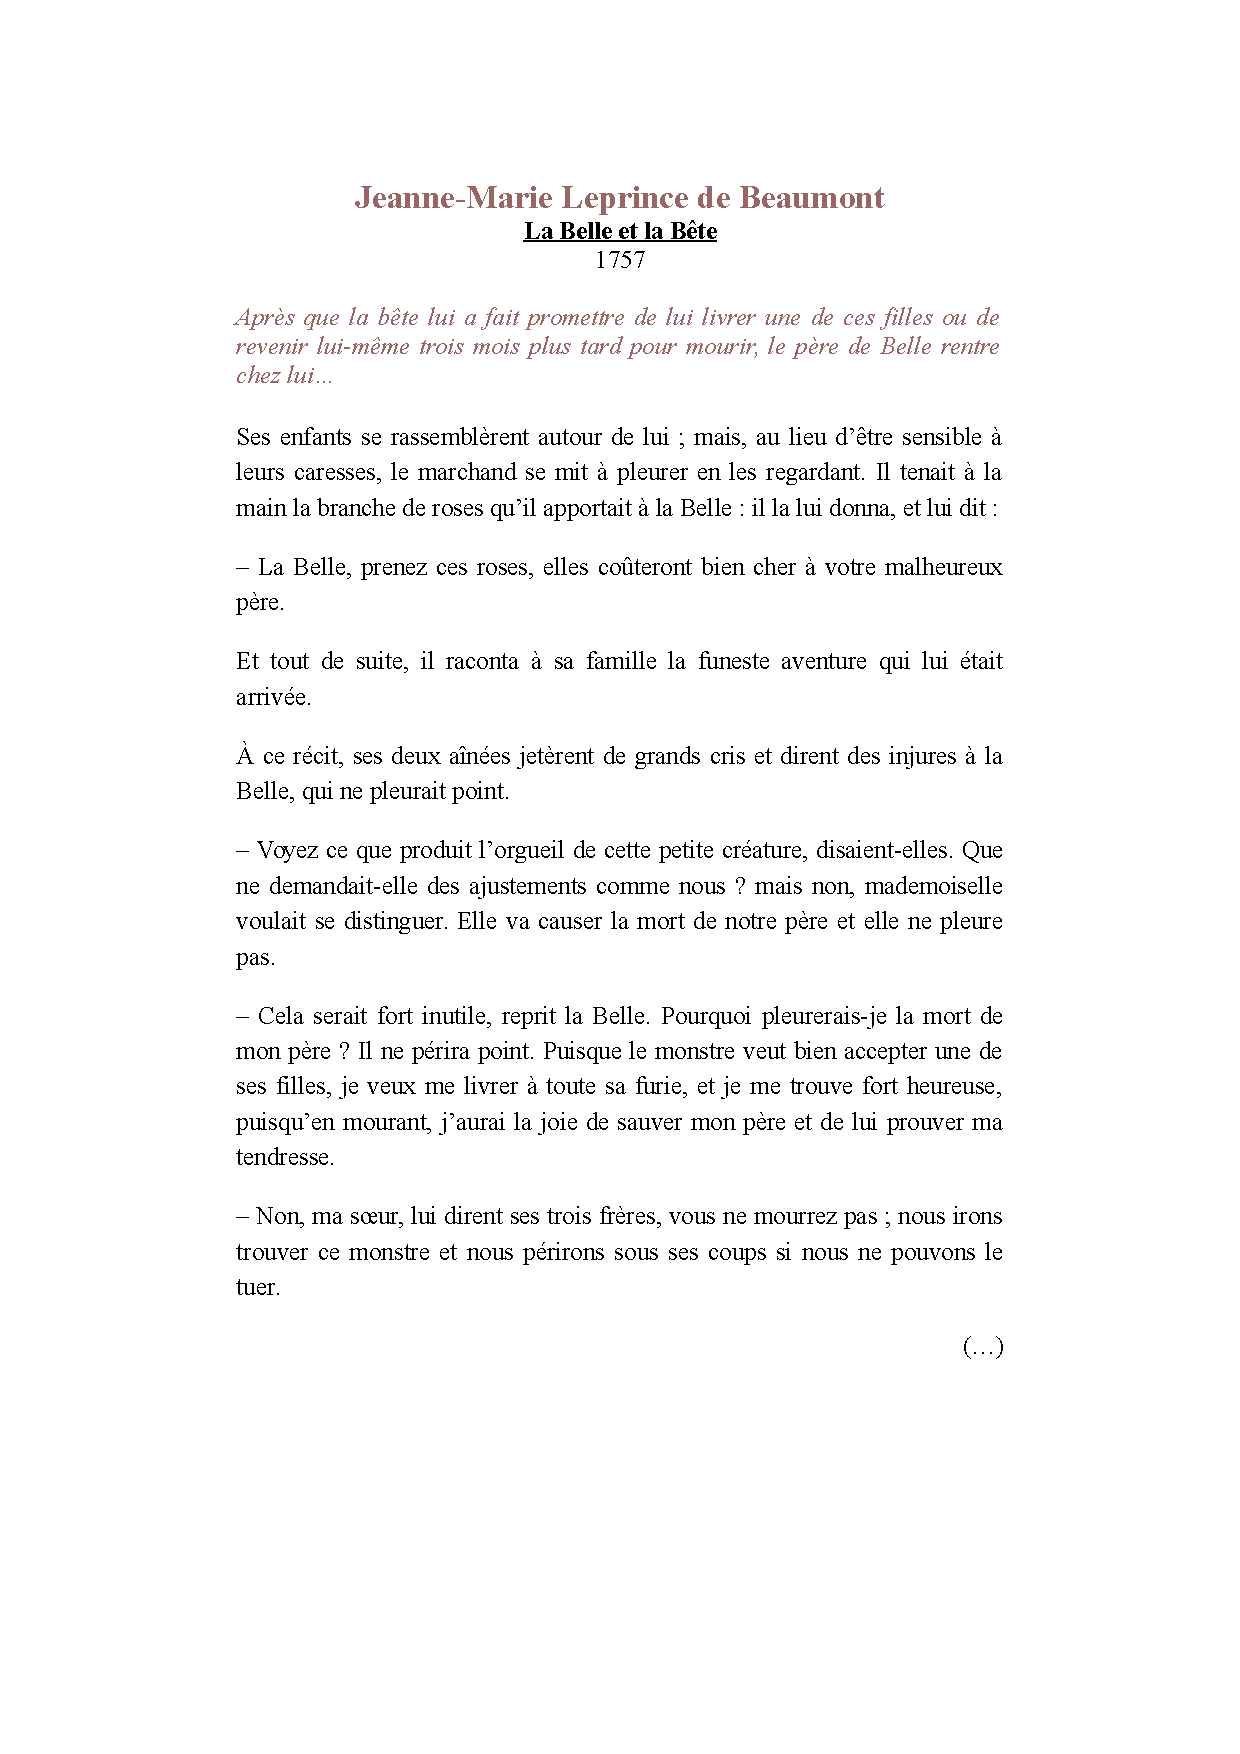
\includegraphics[width=.8\textwidth]{./sources/texte01/LaBelleEtLaBeteFormatee}}\label{modelePage}\end{center}



\textbf{Pour obtenir de l'aide, rendez-vous à la page \pageref{correction_texte01}}


\subsection{Pour aller plus loin...}  

Quand les textes deviennent très longs, il est difficile d'y retrouver un mot en particulier. Les traitements de texte disposent donc d'un outil permettant de rechercher un mot.\index{Writer!Rechercher}\index{Rechercher (Writer)} 

Lorsqu'on souhaite retrouver un mot dans une page de texte, on peut utiliser le raccourci clavier \texttt{cmd + F} :\index{Raccourci Clavier! Cmd + F, rechercher (Writer)}   

\uneimageici{./images/generales/clavierCmdF}{.35\textwidth}

Une barre de recherche s'ouvre alors en haut de la fenêtre :

\uneimageici{./images/texte/WordBarreRecherche.png}{.9\textwidth}

Essayez de rechercher le mot \emph{Belle} : il suffit d'entrer le mot dans la zone de saisie, puis d'appuyer sur la touche \texttt{Entrée}. Pour fermer la barre de recherche, utilisez de nouveau le raccourci clavier \texttt{cmd + F}.   










\poubelle{


%
%
%  S  É  A  N  C  E     II
%
%


\section{Séance 2 : mise en forme d'un texte de J. Swift}\label{ficheTexte2}

\subsection{L'activité demandée}

\prof{l'anglais est enseigné en groupes de niveau et il était difficile de trouver un texte qui soit valable pour tous les groupes. N'hésitez pas à vous approprier cette séance en proposant votre propre texte à votre groupe. Si vous souhaitez faire cette activité avec un texte différent, il suffit de fournir aux élèves (i) le texte brut non mis en forme, (ii) le modèle à atteindre. Ainsi vous pourrez mieux intégrer cette séance à votre progression.}  



\boiteEnonce{Le but de cet exercice est de mettre en forme un extrait d'une œuvre de Jonathan Swift, \emph{Gulliver's travels}, dont une version <<\,brute\,>> est disponible sur la page \emph{Teams} de votre cours. Le modèle à obtenir est montré ci-dessous. Essayez par vous-mêmes de trouver comment faire en testant les possibilités du logiciel.}


\begin{center}\fbox{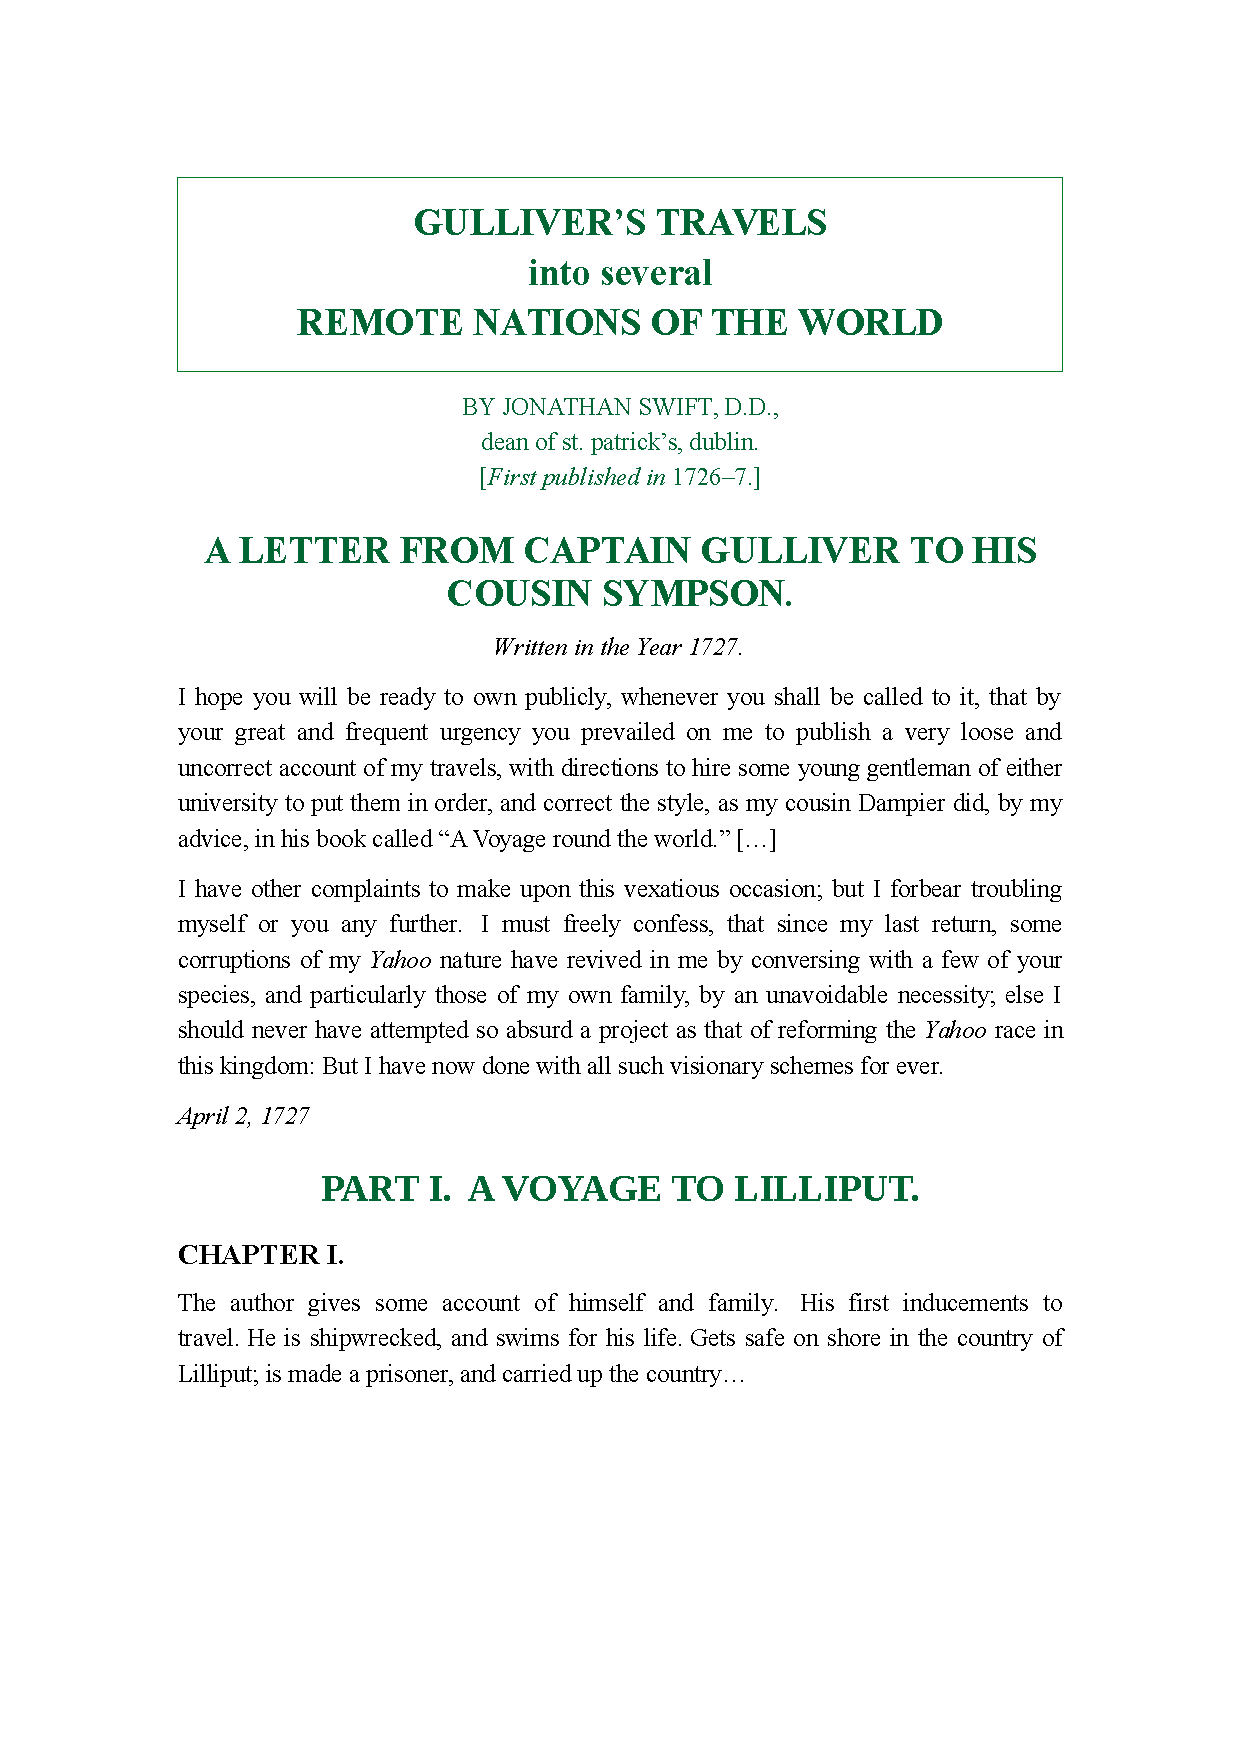
\includegraphics[width=.75\textwidth]{./sources/texte01/ExtraitGulliver6eFormate}}\label{modelePage}\end{center}

\boiteEnonce{Pour parvenir à ce résultat, vous devrez utiliser deux nouvelles fonctionnalités du traitement de texte : passer le texte en majuscule et encadrer un paragraphe. Les opérations à effectuer pour y parvenir sont les suivantes :
\begin{itemize}
\item marges de 3\,cm à gauche, à droite, en haut et en bas ;
\item police de caractères \emph{Times New Roman} ;  
\item titres en caractères de taille 16 points et de couleur \emph{Turquoise} ;
\item texte en caractères de taille 12 points avec un interligne fixe de 0,6\,cm et un espace sous les paragraphes de 0,25\,cm ;
\item quelques parties du texte en italique ; 
\item le texte justifié et les titres centrés.
\end{itemize}}

\boiteEnonce{Une fois la mise en forme terminée, vous devrez exporter votre fichier au format PDF (le fichier doit être nommé à partir de votre nom : \texttt{Nom-date.pdf}) et le rendre sur \emph{Teams} à l'endroit indiqué par votre enseignant.}

\textbf{Pour obtenir de l'aide, rendez-vous à la page \pageref{correction_texte02}}



%
%
%  S  É  A  N  C  E     III
%
%


\section{Séance 3 : mise en forme d'un compte rendu}\label{ficheTexte3}

\prof{cette séance doit être faite sur deux périodes si les élèves préparent eux-mêmes leur compte rendu d'expérience (une période pour la rédaction du compte rendu, et une pour la mise en forme). Il est également possible (comme pour les séances 1 et 2 ci-dessus) de leur donner le compte rendu de la dernière expérience faite, mais non mis en forme, ainsi qu'un modèle de ce qui est attendu. Il faut prévoir une image à insérer dans le compte rendu (format JPG ou PNG), et la mettre à disposition des élèves sur la page \emph{Teams} de votre cours. Précisez aux élèves vos attentes : mise en page, alignements, espacements, taille des caractères, etc.}  

\subsection{L'activité demandée}

\boiteEnonce{Le but de cet exercice est de mettre en forme un compte rendu d'expérience et d'y insérer une image fournie par votre professeur. Vous devez utiliser les techniques apprises dans cette fiche sur le traitement de texte pour préparer votre document.}

\boiteEnonce{Une fois la mise en forme terminée, vous devrez exporter votre fichier au format PDF (le fichier doit être nommé à partir de votre nom : \texttt{Nom-Prénom-date.pdf}) et le rendre sur la plateforme Teams à l'endroit indiqué par votre enseignant.}

\textbf{Pour obtenir de l'aide, rendez-vous à la page \pageref{correction_texte03}}

}


